\chapter[\textsc{D. Mumford~:} Bi-Extensions of Formal Groups]{BI-EXTENSIONS OF FORMAL GROUPS}\label{art15}

\begin{center}
By~~ David Mumford
\end{center}

\lhead[\thepage]{\textit{Bi-Extensions of Formal Groups}}
\rhead[\textit{D. Mumford}]{\thepage}

\setcounter{pageoriginal}{306}
In\pageoriginale the Colloquium itself, I announced that all abelian varieties can be lifted to characteristic zero. The proof of this, as sketched there, is roughly as follows.
\begin{itemize}
\item[(i)] It suffices to prove that every char $p$ abelian variety is a specialization of a char $p$ abelian variety with multiplicative formal group (an ``ordinary'' abelian variety), since Serre (unpublished) has shown that these admit liftings.

\item[(ii)] A preliminary reduction of the problem was made to abelian varieties $X$ such that the invariant
$$
\alpha(X)=\dim_{k}\Hom (\alpha_{p},X)
$$
is $1$.

\item[(iii)] A method was found to construct deformations of a polarized abelian variety from deformations of its polarized Dieudonn\'e module.

\item[(iv)] Finally, some simple deformations of polarized Dieudonn\'e modules were constructed to establish the result.
\end{itemize}

However, it seems premature to give this proof here, since the basic method used in (iii) promises to give much fuller information on the local structure of the formal moduli space of a polarized abelian variety, and this would make my {\em ad hoc} method obsolete. I want instead to give some basic information on the main new technical tool which is used in (iii).

\section{Cartier's result.}\label{art15-sec1}

In the note \cite{art15-key1}, Cartier has announced a module-theoretic classification of formal groups over arbitrary ground-rings $R$. We require only the special case where $p=0$ in $R$, which is foreshadowed in Dieudonn'es original paper \cite{art15-key2}, before the category men got a hold of it, modifying the technique until the restriction ``$R$ = perfect field'' came to seem essential.

\begin{defi*}
Let\pageoriginale $R$ be a ring of characteristic $p$. Let $W(R)$ be the ring of Witt vectors over $R$, and let
\begin{align*}
(a_{0},a_{1},a_{2},\ldots)^{\sigma} &= (a^{p}_{0},a^{p}_{1},a^{p}_{2},\ldots),\\[3pt]
(a_{0},a_{1},a_{2},\ldots)^{t} &= (0,a_{0},a_{1},\ldots). 
\end{align*}
Then $A_{R}$ will denote the ring
$$
W(R)[[V]][F]
$$
modulo the relations:
\begin{itemize}
\item[{\rm(a)}] $FV=p$,

\item[{\rm(b)}] $VaF=a^{t}$,

\item[{\rm(c)}] $Fa=a^{\sigma}F$,

\item[{\rm(d)}] $aV=Va^{\sigma}$,
\end{itemize}
for all $a\in W(R)$.
\end{defi*}

\noindent
{\bf Theorem}~(Dieudonn\'e-Cartier).~{\em There is a covariant equivalence of categories between}
\begin{itemize}
\item[{\rm(A)}] {\em the category of commutative formal groups $\Phi$ over $R$, and}

\item[{\rm(B)}] {\em the category of left $A_{R}$-modules $M$ such that}
\begin{itemize}
\item[{\rm(a)}] $\bigcap\limits_{i}V^{i}M=(0)$,

\item[{\rm(b)}] {\em $Vm=0\Rightarrow m=0$, all $m\in M$,}

\item[{\rm(c)}] {\em $M/VM$ is a free $R$-module of finite rank.}
\end{itemize}
\end{itemize}

The correspondence between these 2 categories can be set up as follows. Recall first that a formal group $\Phi/R$ (by which we mean a set of $n$ power series $\phi_{i}(x_{1},\ldots,x_{n};y_{1},\ldots,y_{n})$, $1\leq i\leq n$, satisfying the usual identities, c.f. Lazard \cite{art15-key3}) defines a covariant functor $F_{\Phi}$ from $R$-algebbras $S$ to groups : i.e. $\forall \ S/R$,
$$
F_{\Phi}(S)=\{(a_{1},\ldots,a_{n})|a_{i}\in S, a_{i}\text{~nilpotent}\}
$$
where
\begin{align*}
&(a_{1},\ldots,a_{n})\cdot (b_{1},\ldots,b_{n})\\
&=(\phi_{1}(a_{1},\ldots,a_{n};b_{1},\ldots,b_{n}),\ldots,\phi_{n}(a_{1},\ldots,a_{n};b_{1},\ldots,b_{n})).
\end{align*}
N. B. In what follows, we will often call the functor $F_{\Phi}$ instead of the power series $\Phi$ the formal group, for simplicity.

Let\pageoriginale $\widehat{W}$ be the functor
$$
\left\{
\begin{array}{l}
\widehat{\bfW}=\{(a_{0},a_{1},\ldots)|a_{i}\in S, a_{i}\text{~ nilpotent, almost all~ } a_{i}=0\},\\
\text{gp law } = \text{Witt vector addition.}
\end{array}\right.
$$
Then we attach to the commutative formal group $\Phi$ the set
$$
M=\Hom_{\text{gp. functors/}R}(\widehat{W},F_{\Phi}),
$$
and since $A_{R}\cong \Hom (\widehat{\bfW},\widehat{\bfW})^{0}$, we can endow $M$ with the structure of left $A_{R}$-module. Conversely, to go in the other direction, first note that any $A_{R}$-module $M$ as in the theorem can be resolved:
\begin{equation*}
0\to A^{n}_{R}\xrightarrow{\beta}A^{n}_{R}\xrightarrow{\alpha}M\to 0.\tag{*}
\end{equation*}
In fact, choose $m_{1},\ldots,m_{n}\in M$ whose images $\mod VM$ are a basis of $M/VM$ as $R$-module. Define
$$
\alpha(P_{1},\ldots,P_{n})=\sum\limits^{n}_{i=1}P_{i}m_{i}.
$$
It is easy to check that $Fm_{i}$ can be expanded in the form $\sum\limits^{n}_{j=1}Q_{ij}(V)m_{j}$, $Q_{ij}$ a power series in $V$ with coefficients in $W(R)$. Define
$$
\beta(P_{1},\ldots,P_{n})=\left(\sum\limits^{n}_{i=1}P_{i}\cdot Q_{i1}-\delta_{i1}F,\ldots,\sum\limits^{n}_{i=1}P_{i}\cdot Q_{in}-\delta_{in}F\right).
$$
It is not hard to check that (*) is exact. Then $\beta$ defines a monomorphism of group functors $\beta^{*}:(\widehat{W})^{n}\to (\widehat{W})^{n}$, and let $F$ be the quotient functor $(\widehat{W})^{n}/\beta^{*}(\widehat{W})^{n}$. Then $F$ is isomorphic to $F_{\Phi}$ for one and-up to canonical isomorphism-only one formal group $\Phi$.

Moreover, we get a resolution of the functor $F_{\Phi}$:
$$
0\to (\widehat{W})^{n}\xrightarrow{\beta^{*}}(\widehat{W})^{n}\to F_{\Phi}\to 0.
$$
When $R$ is a perfect field, the above correspondence can be extended to an analogous correspondence between $p$-divisible groups over $R$ and $W(R)[F,V]$-modules of suitable type (c.f. \cite{art15-key4}, \cite{art15-key5}). However,\pageoriginale it does not seem likely at present that such an extension exists for non-perfect $R$'s. This is a key point.

\section{Bi-extensions of abelian groups.}\label{art15-sec2}

Let $A$, $B$, $C$ be 3 abelian groups. $A$ bi-extension of $B\times C$ by $A$ will denote a set $G$ on which $A$ acts freely, together with a map
$$
G\xrightarrow{\pi} B\times C
$$
making $B\times C$ into the quotient $G/A$, together with 2 laws of composition:
\[
\xymatrix@R=.01cm{
+_{1}:\fprod{G}{G}{B}\to G\ar@{=}[ddddd]_-{\text{def}} & ;\quad +_{2}:\fprod{G}{G}{C}\to G\ar@{=}[ddddd]_-{\text{def}}\\
 & & \\
 & & \\
 & & \\
 & & \\
\{(g_{1},g_{2})|\pi(g_{1}),\pi(g_{2})\text{~have}  & \{(g_{1},g_{2})|\pi(g_{1}),\pi(g_{2})\text{~have}\\
\text{same $B$-component}\} & \text{some $C$-component}\}
}
\]
These are subject to the requirement:
\begin{itemize}
\item[(i)] for all $b\in B$, $G'_{b}=\pi^{-1}(b\times C)$ is an abelian group under $+_{1}$, $\pi$ is a surjective homomorphism of $G'_{b}$ onto $C$, and via the action of $A$ on $G'_{b}$, $A$ is isomorphic to the kernel of $\pi$;

\item[(ii)] for all $c\in C$, $G^{2}_{c}=\pi^{-1}(B\times c)$ is an abelian group under $+_{2}$, $\pi$ is a surjective homomorphism of $G^{2}_{c}$ onto $B$, and via the action of $A$ on $G^{2}_{c}$, $A$ is isomorphic to the kernel of $\pi$;

\item[(iii)] given $x$, $y$, $u$, $v\in G$ such that
\begin{align*}
\pi(x) &= (b_{1},c_{1})\\
\pi(y) &= (b_{1},c_{2})\\
\pi(u) &= (b_{2},c_{1})\\
\pi(v) &= (b_{2},c_{2}),
\end{align*}
then 
$$
(x+_{1}y)+_{2}(u+_{1}v)=(x+_{2}u)+_{1}(y+_{2}v).
$$
This\pageoriginale may seem like rather a mess, but please consider the motivating example: let $X$ be an abelian variety over an algebraically closed field $k$, let $\widehat{X}$ be its dual, and let $P$ be the universal, or Poincar\'e, line bundle on over $X\times \widehat{X}$. Then $P_{k}$, the underlying set of closed points of $P$, is a bi-extension of $X_{k}\times \widehat{X}_{k}$ by $k^{*}$!
\end{itemize}

Notice that if $G$ is a bi-extension of $B\times C$ by $A$, then $\pi^{-1}(B\times 0)$ splits canonically into $A\times B$, and $\pi^{-1}(0\times C)$ splits canonically into $A\times C$. In fact, we can lift $B$ to $\pi^{-1}(B\times 0)$ by mapping $b\in B$ to the element of $G$ which is the identity in $\pi^{-1}(b\times C)$; and we can lift $C$ to $\pi^{-1}(0\times C)$ by mapping $c\in C$ to the element of $G$ which is the identity in $\pi^{-1}(B\times c)$.

Bi-extensions can be conveniently described by co-cycles: choose a (set-theoretic) section
\begin{figure}[H]
\centering
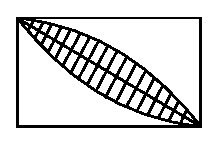
\includegraphics{src/chap15/fig1.eps}
\end{figure}
Via $s$ and the action of $A$ on $G$, we construct an isomorphism
$$
G\cong A\times B\times C
$$
such that the action of $A$ on $G$ corresponds to the action of $A$ on $A\times B\times C$ which is just addition of $A$-components, leaving the $B$-and $C$-components fixed. Then $+_{1}$ and $+_{2}$ go over into laws of composition on $A\times B\times C$ given by:
\begin{align*}
& (a,b,c)+_{1}(a',b,c')=(a+a'+\phi(b;c,c'),b,c+c')\\
& (a,b,c)+_{2}(a',b',c)=(a+a'+\psi (b,b';c),b+b',c).
\end{align*}
For $+_{1}$, $+_{2}$ to be abelian group laws, we need:
\begin{itemize}
\item[(a)] $\phi(b;c+c',c'')+\phi(b;c,c')=\phi(b;c,c'+c'')+\phi(b;c',c'')$

\centerline{$\phi(b;c,c')=\phi(b;c',c);$}

\item[(b)] $\psi(b+b',b'';c)+\psi(b,b';c)=\psi(b,b'+b'';c)+\psi(b',b'';c)$

\centerline{$\psi(b,b';c)=\psi(b',b;c)$.}
\smallskip


The final restriction comes out as:
\item[(c)] $\phi(b+b';c,c')-\phi(b;c,c')-\phi(b';c,c')$\pageoriginale

$=\psi(b,b';c+c')-\psi(b,b';c)-\psi(b,b';c')$.
\end{itemize}
What are the co-boundaries? If you alter $s$ by adding to it a map $\rho:B\times C\to A$, then you check that the new $\phi'$, $\psi'$ are related to the old ones by
\begin{align*}
&\phi'(b;c,c')-\phi(b;c,c')=\rho(b,c+c')-\rho(b,c)-\rho(b,c')\\
&\psi'(b,b';c)-\psi(b,b';c)=\rho(b+b',c)-\rho(b,c)-\rho(b,c).
\end{align*}

Using this explicit expression by co-cycles and co-boundaries, it is clear that the set of all bi-extensions of $B\times C$ by $A$ forms itself an abelian group, which we will denote
$$
\text{Bi-ext~}(B\times C,A).
$$

It is also clear, either from the definition or via co-cycles, that Bi-ext is a covariant functor in $A$, and a contravariant functor in $B$ and $C$.

\section{Bi-extensions of group-functors.}\label{art15-sec3}

\begin{defi*}
If $F$, $G$, $H$ are $3$ covariant functors from the category of $R$-algebras to the category of abelian groups, a bi-extension of $G\times H$ by $F$ is a fourth functor $K$ such that for every $R$-algebra $S$, $K(S)$ is a bi-extension of $G(S)\times H(S)$ by $F(S)$ and for every $R$-homomorphism $S_{1}\to S_{2}$, the map $K(S_{1})\to K(S_{2})$ is a homomorphism of bi-extensions (in the obvious sense). In particular, if $F$, $G$, $H$ are formal groups, this gives us a bi-extension of formal groups.
\end{defi*}

If $F$, $G$, $H$ are formal groups, it is easy again to compute the bi-extensions $K$ by power series co-cycles. In fact, one merely has to check that:
\begin{itemize}
\item[(i)] there is a functorial section
\begin{figure}[H]
\centering
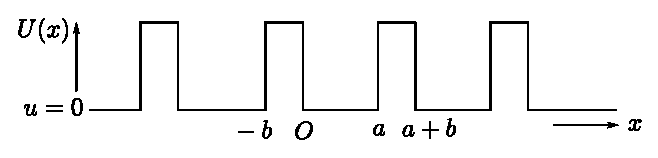
\includegraphics{src/chap15/fig2.eps}
\end{figure}
(this\pageoriginale follows using the ``smoothness'' of the functor $F$, i.e. $F(S)\to F(S/I)$ is surjective if $I$ is a nilpotent ideal);

\item[(ii)] any morphism of functors from one product of formal groups to another such product is given explicitly by a set of power series over $R$ in the appropriate variables.
\end{itemize}

In fact, we will be exclusively interested in the case where $F=\widehat{\bfG}_{m}$ is the formal multiplicative group; that is
$$
\widehat{\bfG}_{m}(S)=
\left\{
\begin{array}{l}
\text{Units in $S$ of form $1+x$, $x$ nilpotent,}\\
\text{composed via multiplication.}
\end{array}
\right\}
$$
Then if $G$ and $H$ are formal groups in variables $x_{1},\ldots,x_{n}$ and $y_{1},\ldots,y_{m}$, a bi-extension of $G\times H$ by $\widehat{\bfG}_{m}$ is given by 2 power series 
$$
\sigma(x_{1},\ldots,x_{n};y_{1},\ldots,y_{m},y'_{1},\ldots,y'_{m}), \tau(x_{1},\ldots,x_{n},x'_{1},\ldots,x'_{n};y_{1},\ldots,y_{m})
$$ 
with constant terms $1$ such that - abbreviating $n$-tuples and $m$-tuples:
\begin{align*}
& \sigma(x;\Phi(y,y'),y'')\cdot \sigma(x;y,y')=\sigma(x;y,\Phi(y',y''))\cdot \sigma (x;y',y'')\\
& \sigma(x;y,y')=\sigma(x;y',y)\\
& \tau (\Psi(x,x'),x'',y)\cdot \tau(x,x';y)=\tau(x,\Psi(x',x'');y)\cdot \tau(x',x'';y)\\
& \tau (x,x';y)=\tau(x',x;y)\\
& \sigma(\Psi(x,x');y,y')\cdot \sigma(x;y,y')^{-1}\cdot \sigma (x';y,y')^{-1}=\tau(x,x';\Phi(y,y'))\cdot\\
&\hspace{5cm} \tau(x,x';y)^{-1}\cdot \tau(x,x';y')^{-1},
\end{align*}
if $\Phi$, $\Psi$ are the group laws of $G$ and $H$ respectively.

We want one slightly non-trivial fact about general bi-extensions. This result gives essentially the method for computing Bi-ext's via resolutions.

\medskip
\noindent
{\bf Proposition \thnum{1}.\label{art15-prop1}}
{\em Let $E$, $G$, $G'$ be abelian group functors as above. Suppose}
\begin{align*}
& 0\to F_{1}\to F_{0}\to G\to 0\\
& 0\to F'_{1}\to F'_{0}\to G'\to 0
\end{align*}
{\em are $2$ exact sequences of such functors. Then}
{\fontsize{10pt}{12pt}\selectfont
\begin{gather*}
\Ker \{\text{\rm Bi-ext }(G\times G',E)\to \text{\rm Bi-ext } (F_{0}\times F'_{0},E)\}\\
\cong \frac{\begin{array}{l}\{(f,g)|f:F_{0}\times F'_{1}\to E\text{~ and~ } g:F_{1}\times F'_{0}\to E\text{\em~ bi-homomorphisms}\\ \res f=\res g\text{~ on~ } F_{1}\times F'_{1}\}\end{array}}{\{(f,g)|\exists h:F_{0}\times F'_{0}\to E\text{\em \ bi-homomorphism,~} f \text{~and~} g \text{~restrictions of~} h\}}
\end{gather*}}\relax\pageoriginale

The proof goes along these lines: let $H$ be a bi-extension of $G\times G'$ by $E$. If it lies in the above kernel, then the induced bi-extension of $F_{0}\times F'_{0}$ is trivial:
$$
\fprod{H}{(F_{0}\times F'_{0})}{(G\times G')}\cong E\times F_{0}\times F'_{0}.
$$
Consider the equivalence relation on the functor $E\times F_{0}\times F'_{0}$ induced by the mapping of it onto $H$. It comes out that there are maps $f:F_{0}\times F'_{1}\to E$, $g:F_{1}\times F'_{0}\to E$ such that this equivalence relation is generated by
\begin{multline}
(a,b,c)\sim (a+f(b,\overline{c}),b,c+\overline{c}),a\in E(S),b\in F_{0}(S)\\
c\in F'_{0}(S),\overline{c}\in F'_{1}(S).\label{art15-eq1}
\end{multline}
and
\begin{multline}
(a,b,c)\sim (a+g(\overline{b},c),b+\overline{b},c), a\in E(S), b\in F_{0}(S)\\
b\in F_{1}(S), c\in F'_{0}(S).\label{art15-eq2}
\end{multline}

Moreover, $f$ and $g$ have to be bi-homomorphisms with $\res f=\res g$ on $F_{1}\times F'_{1}$. Conversely, given such $g$ and $g$, define the functor $H$ to be the quotient of $E\times F_{0}\times F'_{0}$ by the above equivalence relation. $H$ turns out to be a bi-extension. Finally, the triviality of $H$ can be seen to be equivalent to $f$ and $g$ being the restrictions of a bi-homomorphism $h:F_{0}\times F'_{0}\to E$.

\section{Bi-extensions of \texorpdfstring{$\widehat{W}$}{W}.}\label{art15-sec4}

\noindent
{\bf Proposition \thnum{2}.\label{art15-prop2}}
${\rm Bi-ext } (\widehat{\bfW}\times \widehat{\bfW},\widehat{\bfG}_{m})=(0)$.

\begin{proof}
Consider functors $F$ from ($R$-algebras) to (abelian groups) which are isomorphic as set functors to $D^{I}$, where
$$
D^{I}(S)=\{(a_{i})|a_{i}\in S,\text{ all } i\in I, a_{i}\text{ nilpotent, almost all } a_{i}=0\}
$$
and where $I$ is an indexing set which is either finite or countably infinite. Note that all our functors are of this type. Then I claim that for all $R$ of char $p$, all such $F$, there is a canonical retraction $p_{F}$:
\begin{figure}[H]
\centering
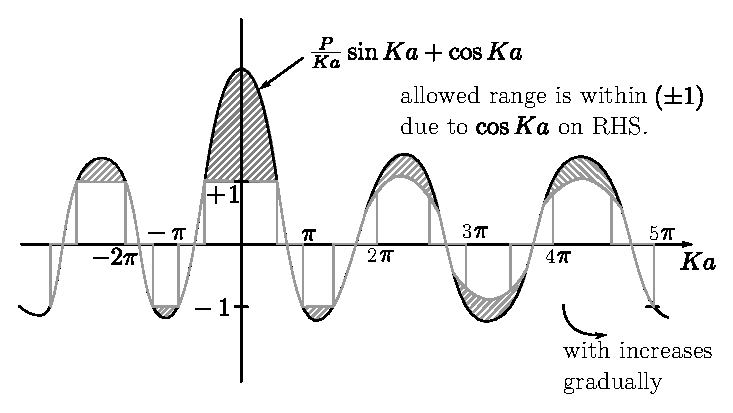
\includegraphics{src/chap15/fig3.eps}
\end{figure}\pageoriginale
which is functorial both with respect to \eqref{art15-eq1} any homomorphism $F\to G$, and \eqref{art15-eq2} base changes $R_{1}\to R_{2}$.

The construction of $p_{F}$ is based on Theorem 1 of Cartier's note \cite{art15-key1}. Let $\widehat{W}^{*}$ be the full Witt group functor (i.e. based on all positive integers, rather than powers of $p$), and let $i:D\to \widehat{\bfW}^{*}$ be the canonical inclusion used in \cite{art15-key1}. Then Theorem 1 asserts that for all formal groups $F$, every morphism $\phi:D\to F$ extends uniquely to a homomorphism $u:\widehat{\bfW}^{*}\to F$.
\[
\xymatrix@=1.5cm{
D\ar[r]^-{\phi}\ar@{_(->}[d]_-{i} & F\\
\widehat{\bfW}^{*}\ar@{-->}[ur]_-{u}
}
\]
Cartier informs me that this theorem extends to all $F$'s of our type. On the other hand, $\widehat{\bfW}$, over a ring of char $p$, is a direct summand of $\widehat{\bfW}^{*}$:
\[
\xymatrix@C=1.5cm{
\widehat{\bfW}^{*}\ar@<-.3pc>[r]_-{\pi} & \widehat{\bfW}\ar@<-.3pc>[l]_{j}.
}
\]
Construct $p_{F}$ as follows: given $f:\widehat{\bfW}\to F$, let $\phi=\res$ to $D$ of $f\circ \pi$; let $u$ = extension of $\phi$ to a homomorphism $u$; let $p_{F}(f)=u\circ j$.

Now let $F$ be a bi-extension of $\widehat{\bfW}\times \widehat{\bfW}$ by $\widehat{\bfG}_{m}$. For every $R$-algebra $S$ and every $a\in \widehat{\bfW}(S)$, let $F'_{a}$ (resp. $F''_{a}$) denote the fibre functor of $F$ over $\{a\}\times \widehat{\bfW}$ (resp. $\widehat{\bfW}\times \{a\}$) (i.e. $F_{a}(T)=\{b\in F(T)|1^{\text{st}}$ (resp. $2^{\text{nd}}$) component of $\pi(b)$ is induced by $a$ via $S\to T$\}). Then $F'_{a}$ and $F''_{a}$ are group\pageoriginale functors of the good type extending $\widehat{\bfW}$ by $\widehat{\bfG}_{m}$ over ground ring $S$. Now since $\widehat{\bfG}_{m}$ is smooth, one can choose a section $s$ to $\pi$:
\begin{figure}[H]
\centering
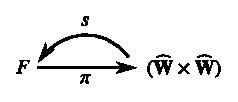
\includegraphics{src/chap15/fig4.eps}
\end{figure}
$s$ restricts to morphisms $s_{a}:\widehat{W}/S\to F'_{a}$, for all $a\in \widehat{\bfW}(S)$. Take $p_{F'_{a}}(s_{a})$. As $a$ varies, these fit together into a new section $p'(s)$ to $\pi$. But $p'(s)$ is now a homomorphism with respect to addition into the $2^{\text{nd}}$ variable, i.e.
\begin{equation*}
p'(s)(u,v)+_{1}p'(s)(u,v')=p'(s)(u,v+v').\tag*{(*)$'$}
\end{equation*}
Now switch the 2 factors : $p'(s)$ restricts to morphism $p'(s)_{a}:\widehat{\bfW}/S\to F''_{a}$, for all $a\in \widehat{\bfW}(S)$. Take $p_{F''_{a}}(p'(s)_{a})$. As $a$ varies, these fit together into a new section $p''(p'(s))$ to $\pi$.

Then this satisfies :
\begin{equation*}
p''(p'(s))(u,v)+_{2}p''(p'(s))(u',v)=p''(p'(s))(u+u',v).\tag*{(*)$''$}
\end{equation*}
But now, using the functoriality of $p$, and the property of bi-extensions linking $+_{1}$ and $+_{2}$, it falls out that $p''(p'(s))$ still has property $(*)'$ enjoyed by $p'(s)$! So $p''(p'(s))$ preserves both group laws and splits the extension $F$.
\end{proof}

\begin{defi*}
$\overline{A}_{R}$ will denote the ring $W(R)[[F,V]]$ modulo the relations
\begin{itemize}
\item[\rm(a)] $FV=p$

\item[\rm(b)] $VaF=a'$

\item[\rm(c)] $Fa=a^{\sigma}F$

\item[\rm(d)] $aV=Va^{\sigma}$, \ \ all $a\in W(R)$.
\end{itemize}
\end{defi*}
Every element in this ring can be expanded uniquely in the form:
$$
P=a_{0}+\sum\limits^{\infty}_{i=1}V^{i}a_{i}+\sum\limits^{\infty}_{i=1}a_{-i}F^{i}.
$$
For every such $P$, let
$$
P^{*}=a_{0}+\sum\limits^{\infty}_{i=1}a_{i}F^{i}+\sum\limits^{\infty}_{i=1}V^{i}a_{-i}.
$$\pageoriginale
Then * is an anti-automorphism of $\overline{A}_{k}$ of order 2. We shall consider $\overline{A}_{R}$ as an $A_{R}\times A_{R}$-module via
\begin{equation*}
(P,Q)\cdot x=P\cdot x\cdot Q^{*}.\tag{*}
\end{equation*}

\smallskip
\noindent
{\bf Proposition \thnum{3}.\label{art15-prop3}}
$\text{\rm Bi-hom}_{R} (\widehat{\bfW}\times \widehat{\bfW},\widehat{\bfG}_{m})\cong \overline{A}_{R}$.

\smallskip
\noindent
{\em Moreover, since $A_{R}=\Hom_{R}(\widehat{\bfW},\widehat{\bfW})^{0}$, the left-hand side is an $A_{R}\times A_{R}$-module; under the above isomorphism, this structure corresponds to the $A_{R}\times A_{R}$-module structure on $\overline{A}_{R}$ defined by $(*)$.}

\begin{proof}
Cartier \cite{art15-key1} has shown that for all $R$, the Artin-Hasse exponential defines isomorphisms
$$
\Hom_{R}(\widehat{\bfW},\widehat{\bfG}_{m})\cong \bfW(R)
$$
where $\bfW$ is the full Witt functor
$$
\left\{
\begin{array}{l}
\bfW(R)=\{(a_{0},a_{1},\ldots)|a_{i}\in R\}\\
\text{group law = addition of Witt vectors.}
\end{array}
\right.
$$
Therefore,
$$
\text{\rm Bi-Hom}_{R}(\widehat{\bfW}\times \widehat{\bfW}, \widehat{G}_{m})\cong \Hom_{R}(\widehat{\bfW},\bfW).
$$
Define a homomorphism
\begin{align*}
&\overline{A}_{R}\xrightarrow{\phi}\Hom_{R}(\widehat{\bfW},\bfW)\\
\text{by}\qquad & P\to \text{the map } [b\mapsto P(b)].
\end{align*}
Here $P(b)$ means that $V$ and $F$ operate on Witt vectors in the usual way: note that the doubly infinite series $P$ operators on $b$ since $b$ has only a finite number of components and all are nilpotent, whereas $P(b)$ is allowed to have all components non-zero.

Let
$$
\widehat{\bfW}_{n}(R)=\{(a_{0},a_{1},\ldots)|a^{p^{n}}_{i}=0,\text{~ all~ } i;\text{~ almost all~ } a_{i}=0\}.
$$
Notice that
$$
\Hom_{R}(\widehat{\bfW},\bfW)\cong \varprojlim_{n}\Hom_{R}(\widehat{\bfW}_{n},\bfW),
$$
and\pageoriginale that $\phi$ factors through maps
$$
\overline{A}_{R}/\overline{A}_{R}\cdot F^{n}\xrightarrow{\phi_{n}}\Hom_{R}(\widehat{\bfW}_{n},\bfW).
$$
It suffices to show that $\phi_{n}$ is an isomorphism for all $n$. But for $n=1$, $\overline{A}_{R}/\overline{A}_{R}\cdot F\cong R[[V]]$, while
$$
\Hom_{R}(\widehat{\bfW}_{1},\bfW)\cong \Hom_{p\text{-Lie algebras}}(\Lie (\widehat{\bfW},\Lie(\bfW)).
$$
Also $\Lie(\widehat{\bfW})$ is the free $R$-module on generators $\widehat{e}_{0}$, $\widehat{e}_{1}$, $\widehat{e}_{2},\ldots$ with $\widehat{e}_{i}^{(p)}=\widehat{e}_{i+1}$; and $\Lie(\bfW)$ is the $R$-module of all expressions $\sum\limits^{\infty}_{i=0}a_{i}e_{i}$, $a_{i}\in R$, with same $p^{\text{th}}$ power map. Moreover $\sum\limits^{\infty}_{i=0} V^{i}a_{i}\in R[[V]]$ goes via $\phi_{1}$ to the lie algebra map taking $\widehat{e}_{0}$ to $\sum\limits^{\infty}_{i=0}a_{i}e_{i}$. Thus $\phi_{1}$ is an isomorphism. Now use induction on $n$, and the exact sequences 
$$
0\to \widehat{\bfW}_{n-1}\to \widehat{\bfW}_{n}\xrightarrow{F^{n-1}}\widehat{\bfW}_{1}\to 0.
$$
This leads to the diagram:
\[
\xymatrix{
0\ar[r] & \Hom_{R}(\widehat{\bfW}_{1},\bfW)\ar[r]^-{\circ F^{n-1}} & \Hom_{R}(\widehat{\bfW}_{n},\bfW)\ar[r] & \Hom_{R}(\widehat{\bfW}_{n-1},\bfW)\\
0\ar[r] & \overline{A}_{R}/\overline{A}_{R}\cdot F\ar[r]^-{\times F^{n-1}}\ar[u]_-{\phi_{1}} & \overline{A}_{R}/\overline{A}_{R}\cdot F^{n}\ar[u]_-{\phi_{n}}\ar[r] & \overline{A}_{R}/\overline{A}_{R}\cdot F^{n-1}\to 0.\ar[u]_-{\phi_{n-1}}  
}
\]
The bottom line is easily seen to the exact, so if $\phi_{1}$ and $\phi_{n-1}$ are isomorphisms, the diagram implies that $\phi_{n}$ is an epimorphism.
\end{proof}

\begin{coro*}
Let $F_{1}$ and $F_{2}$ be group functors isomorphic to $(\widehat{\bfW})^{n_{i}}$ for some $n_{1}$, $n_{2}$. Let $M_{i}=\Hom_{R}(\widehat{\bfW},F_{i})$ be the corresponding finitely generated, free $A_{R}$-module. Then there is a $1-1$ correspondence between bi-homomorphisms
$$
B:F_{1}\times F_{2}\to \widehat{\bfG}_{m}
$$
and maps
$$
\beta : M_{1}\times M_{2}\to \overline{A}_{R},
$$\pageoriginale
bi-linear in the following sense:
$$
\beta (Pm,Qn)=P\cdot (m,n)\cdot Q^{*}
$$
(all $m\in M_{1}$, $n\in M_{2}$, $P$, $Q\in A_{R}$).
\end{coro*}

\section{Applications.}\label{art15-sec5}

Putting Propositions \ref{art15-prop1}, \ref{art15-prop2} and \ref{art15-prop3} together, we conclude the followng

\begin{coro*}
\begin{itemize}
\item[(a)] Let $\Phi$, $\Psi$ be formal groups over $R$.

\item[(b)] Let $M$, $N$ be the corresponding Dieudonn\'e modules.

\item[(c)] Let
\begin{align*}
& 0\to F_{1}\to F_{0}\to M\to 0\\
& 0\to G_{1}\to G_{0}\to N\to 0
\end{align*}
be resolutions of $M$ and $N$ by finitely generated, free $A_{R}$-modules. Then the group ${\rm Bi-ext}_{R}(\Phi\times \Psi, \widehat{\bfG}_{m})$ of bi-extensions of formal groups can be computed as the set of pairs of bi-linear maps:
\begin{align*}
& \beta : F_{0}\times G_{1}\to \overline{A}_{R},\\
& \gamma : F_{1}\times G_{0}\to \overline{A}_{R},
\end{align*}
such that $\beta=\gamma$ on $F_{1}\times G_{1}$, taken modulo restrictions of bi-linear maps $\alpha : F_{0}\times G_{0}\to \overline{A}_{R}$.
\end{itemize}
\end{coro*}

In another direction, bi-extensions can be linked to $p$-divisible\break groups, as defined by Take \cite{art15-key6}.

\medskip
\noindent
{\bf Proposition \thnum{4}.\label{art15-prop4}}
{\em Let $F$ and $F'$ be formal groups over a {\rm char} $p$ ring $R$. Assume that the subgroups $G_{n}$(resp. $G'_{n}$) = $\Ker (p^{n}\text{~ in~ } F(\text{resp } F'))$ form $p$-divisible groups over $R$(i.e. $F$ and $F'$ are ``equi-dimensional'', or of ``finite height''). Then there is a $1-1$ correspondence between {\rm(1)} bi-extensions of $F\times F'$ by $\widehat{G}_{m}$ and {\rm(2)} sets of bi-homomorphisms $\beta_{n}:G_{n}\times G'_{n}\to \mu_{p^{n}}$, such that for all $x\in G_{n+1}(S)$, $y\in G'_{n+1}(S)$,}
$$
\beta_{n}(px,py)=\beta_{n+1}(x,y)^{p}.
$$

\begin{proof}
We\pageoriginale will use descent theory and existence of quotients by finite, flat equivalence relations: c.f. Raynaud's article in the same volume as Tate's talk \cite{art15-key6}. Starting with the $\beta_{n}$'s, let $L_{n}$ be the quotient functor in the flat topology of $\widehat{\bfG}_{m}\times G_{n}\times G'_{2n}$ by the equivalence relation:
$$
(\lambda,x,y)\sim (\lambda\cdot \beta_{n}(x,b),x,y+b)
$$
where $\lambda\in \widehat{\bfG}_{m}(S)$, $x\in G_{n}(S)$, $y\in G'_{2n}(S)$, $b\in G'_{n}(S)$. Then $L_{n}$ is a bi-extension of $G_{n}\times G'_{n}$ by $\widehat{G}_{m}$. Moreover, $L_{n}$ is a subfunctor of $L_{n+1}$, so if we let $L$ be the direct limit of the functor $L_{n}$, then $L$ is a bi-extension of $F\times F'$ by $\widehat{\bfG}_{m}$.

Conversely, if we start with $L$, let $L_{n}$ be the restriction of $L$ over $G_{n}\times G'_{n}$. In the diagram
\[
\xymatrix@C=3cm{
& L_{n}\ar[d]^-{\pi}\\
G_{n}\times G'_{2n}\ar@{-->}[ur]^-{\phi}\ar[r]_-{1\times p^{r}} & G_{n}\times G'_{n},
}
\]
I want to define a canonical map $\phi$ which is a homomorphism in both variables, i.e. which splits the induced bi-extension over $G_{n}\times G'_{2n}$. Suppose $x\in G_{n}(S)$, $y\in G'_{n}(S)$ for some $R$-algebra $S$. Choose $z_{1}\in L(S)$ such that $\pi(z_{1})=(x,y)$. If we add $z_{1}$ to itself $p^{n}$ times in the $1^{\text{st}}$ variable, we obtain a point:
\begin{align*}
& [p^{n}]_{+_{1}}(z_{1})=z_{2}\\
& \pi(z_{2})=(0,y).
\end{align*}
But $\pi^{-1}((0\times F')$ is canonically isomorphic to $\widehat{\bfG}_{m}\times (0)\times F'$, so $z_{2}=(\lambda,0,y)$, some $\lambda\in \widehat{\bfG}_{m}(S)$. Now choose a finite flat $S$-algebra $S'$ such that $\lambda=\mu^{p_{n}}$ for some $\mu\in \widehat{\bfG}_{m}(S')$. Letting $z_{1}$ also denote the element of $L(S')$ induced by $z_{1}$, define $z'_{1}=\mu^{-1}\cdot z_{1}$. This is a new point of $L$ over $(x,y)$, which now satisfies $[p^{n}]_{+_{1}}(z'_{1})=(1,0,y)$. Now add $z'_{1}$ to itself $p^{n}$ times in the $2^{\text{nd}}$ variable. This gives a point
\begin{gather*}
[p^{n}]_{+_{2}}(z'_{1})=z'_{3}\in L^{*}_{n}(S'),\\
\pi(z'_{3})=(x,p^{n}y).
\end{gather*}\pageoriginale
Clearly, $z'_{3}$ is independent of the choice of $\mu$, so by descent theory, $z'_{3}$ must be induced by a unique element $z_{3}\in L_{n}(S)$. Define $\phi(x,y)=z_{3}$. It is easy to check that $\phi$ is a homomorphism in both variables.

We can use $\phi$ to set up a fibre product diagram:
\[
\xymatrix@=1.2cm{\widehat{\bfG}_{m}\times G_{n}\times G'_{2n}\ar[d]^-{\pi}\ar[r]^-{\alpha} & L_{n}\ar[d]^-{\pi}\\
G_{n}\times G'_{2n}\ar[r]_-{(1\times p^{n})} & G_{n}\times G'_{n}
}
\]
where $\alpha$ is a homomorphism of bi-extensions. Since $p^{n}$ is faithfully flat, so is $\alpha$, and $L_{n}$ is therefore the quotient of $\widehat{\bfG}_{m}\times G_{n}\times G'_{2n}$ by a suitable flat equivalence relation. For every $x\in G_{n}(S)$, $y\in G'_{2n}(S)$, $b\in G'_{n}(S)$ and $\lambda\in \widehat{\bfG}_{m}(S)$, there is a unique element $\beta_{n}(x,y,b,\lambda)\in \widehat{\bfG}_{m}(S)$ such that
$$
\alpha((\lambda,x,y))=\alpha((\lambda\cdot \beta_{n}(x,y,b,\lambda),x,y+b)
$$
and this function $\beta_{n}$ describes the equivalence relation. Using the fact that $\alpha$ is a homomorphism of bi-extensions, we deduce
\begin{itemize}
\item[(1)] that $\beta_{n}$ does not depend on $\lambda$,

\item[(2)] $\beta_{n}(x,y,b)\cdot \beta_{n}(x,y+b,b')=\beta_{n}(x,y,b+b')$ (via associativity of equivalence relation),

\item[(3)] $\beta_{n}(x,y,b)\cdot \beta_{n}(x',y,b)=\beta_{n}(x+x',y,b)$ ($\alpha$ preserves $+_{1}$),

\item[(4)] $\beta_{n}(x,y,b)\cdot \beta_{n}(x,y',b')=\beta_{n}(x,y+y',b+b')$ ($\alpha$ preserves $+_{2}$).
\end{itemize}
By (4) and (2) with $b=y'=0$,
$$
\beta_{n}(x,y,0)\cdot \beta_{n}(x,0,b')=\beta_{n}(x,y,b')=\beta_{n}(x,y,0)\cdot \beta_{n}(x,y,b'),
$$
hence $\beta_{n}$ is independent of $y$ too. Then (3) and (4) show that $\beta_{n}$ is a bi-homomorphism, so $L_{n}$ is constructed from a $\beta_{n}$ as required. We\pageoriginale leave it to the reader to check that if we start from a set of $\beta_{n}$'s, and construct a bi-extension $L$, then the above procedure leads you back to these same $\beta_{n}$'s.
\end{proof}

I think that with these results, bi-extensions can be applied to the problem of determining the local structure of the moduli space of polarized abelian varieties.

\begin{thebibliography}{99}
\bibitem{art15-key1} \textsc{P. Cartier :} Modules associ\'es \`a un groupe formel commutatif, {\em Comptes Rendus Acad. France,} Series A, 265 (1967), 129.

\bibitem{art15-key2} \textsc{J. Dieudonn\'e :} Lie groups and Lie hyperalgebras over a field of char. $p$, {\em Amer. J. Math.} 77 (1955), p. 203.

\bibitem{art15-key3} \textsc{M. Lazard :} Lois de groupes et analyseurs, {\em Ann. Ecoles Normales Sup.} 72 (1955), p. 299, 

\bibitem{art15-key4} \textsc{Y. Manin :} Theory of commutative formal groups over fields of finite characteristic, {\em Usp. Math. Nauk,} 18 (1963), p. 3 (English transl. : {\em Russian Math. Surveys,} 18, p. 1).

\bibitem{art15-key5} \textsc{T. Oda :} {\em Abelian Varieties and Dieudonn\'e Modules,} Thesis, Harvard University, 1967.

\bibitem{art15-key6} \textsc{J. Tate :} $p$-divisible groups, in {\em Local Fields}, Springer-Verlag, 1967.

\end{thebibliography}

\bigskip

\noindent
{\small Tata Institute of Fundamental Research}

\noindent
{\small Bombay}
